\def\paperversiondraft{draft}
\def\paperversionnormal{normal}

% If the paper version is set to 'normal' mode keep it,
% otherwise set it to 'draft' mode.
\ifx\paperversion\paperversionnormal
\else
  \def\paperversion{draft}
\fi

\documentclass[review, acmsmall, nonacm]{acmart}

\def\acmversionanonymous{anonymous}
\def\acmversionjournal{journal}
\def\acmversionnone{none}

\makeatletter
\if@ACM@anonymous
  \def\acmversion{anonymous}
\else
  \def\acmversion{journal}
\fi
\makeatother

\usepackage{colortbl}

% 'draftonly' environment
\usepackage{environ}
\ifx\paperversion\paperversiondraft
\newenvironment{draftonly}{}{}
\else
\NewEnviron{draftonly}{}
\fi

% Most PL conferences are edited by conference-publishing.com. Follow their
% advice to add the following packages.
%
% The first enables the use of UTF-8 as character encoding, which is the
% standard nowadays. The second ensures the use of font encodings that support
% accented characters etc. (Why should I use this?). The mictotype package
% enables certain features 'to­wards ty­po­graph­i­cal per­fec­tion
\usepackage[utf8]{inputenc}
\usepackage[T1]{fontenc}
\usepackage{microtype}

\usepackage{xargs}
\usepackage{lipsum}
\usepackage{xparse}
\usepackage{xifthen, xstring}
\usepackage{xspace}
\usepackage{marginnote}
\usepackage{etoolbox}
\usepackage[acronym,shortcuts]{glossaries}
\usepackage{amsmath}
\usepackage{thmtools} % required for autoref to lemmas
\usepackage{algorithm}
\usepackage[noend]{algpseudocode}
\usepackage{hyphenat}
\usepackage[shortcuts]{extdash}

\input{tex/setup.tex}
\input{tex/acm.tex}

\usemintedstyle{colorful}

% Newer versions of minted require the 'customlexer' argument for custom lexers
% whereas older versions require the '-x' to be passed via the command line.
\makeatletter
\ifcsdef{MintedExecutable}
{
  % minted v3
  \newminted[mlir]{tools/lexers/MLIRLexer.py:MLIRLexerOnlyOps}{mathescape}
  \newminted[xdsl]{tools/lexers/MLIRLexer.py:MLIRLexer}{mathescape, style=murphy}
  \newminted[lean4]{tools/lexers/Lean4Lexer.py:Lean4Lexer}{mathescape}
}
{
  \ifcsdef{minted@optlistcl@quote}
  {
    \newminted[mlir]{tools/lexers/MLIRLexer.py:MLIRLexerOnlyOps}{customlexer, mathescape}
    \newminted[xdsl]{tools/lexers/MLIRLexer.py:MLIRLexer}{customlexer, mathescape, style=murphy}
    \newminted[lean4]{tools/lexers/Lean4Lexer.py:Lean4Lexer}{customlexer, mathescape}
  }
  {
    \newminted[mlir]{tools/lexers/MLIRLexer.py:MLIRLexerOnlyOps -x}{mathescape}
    \newminted[xdsl]{tools/lexers/MLIRLexer.py:MLIRLexer -x}{mathescape, style=murphy}
    \newminted[lean4]{tools/lexers/Lean4Lexer.py:Lean4Lexer -x}{mathescape}
  }
}
\makeatother

% We use the following color scheme
%
% This scheme is both print-friendly and colorblind safe for
% up to four colors (including the red tones makes it not
% colorblind safe any more)
%
% https://colorbrewer2.org/#type=qualitative&scheme=Paired&n=4

\definecolor{pairedNegOneLightGray}{HTML}{cacaca}
\definecolor{pairedNegTwoDarkGray}{HTML}{827b7b}
\definecolor{pairedOneLightBlue}{HTML}{a6cee3}
\definecolor{pairedTwoDarkBlue}{HTML}{1f78b4}
\definecolor{pairedThreeLightGreen}{HTML}{b2df8a}
\definecolor{pairedFourDarkGreen}{HTML}{33a02c}
\definecolor{pairedFiveLightRed}{HTML}{fb9a99}
\definecolor{pairedSixDarkRed}{HTML}{e31a1c}

\createtodoauthor{grosser}{pairedOneLightBlue}
\createtodoauthor{ivan}{pairedTwoDarkBlue}
\createtodoauthor{authorThree}{pairedThreeLightGreen}
\createtodoauthor{authorFour}{pairedFourDarkGreen}
\createtodoauthor{authorFive}{pairedFiveLightRed}
\createtodoauthor{authorSix}{pairedSixDarkRed}

\newacronym{ir}{IR}{Intermediate Representation}

\graphicspath{{./images/}}

% Define macros that are used in this paper
%
% We require all macros to end with a delimiter (by default {}) to enusure
% that LaTeX adds whitespace correctly.
\makeatletter
\newcommand\requiredelimiter[2][########]{%
  \ifdefined#2%
    \def\@temp{\def#2#1}%
    \expandafter\@temp\expandafter{#2}%
  \else
    \@latex@error{\noexpand#2undefined}\@ehc
  \fi
}
\@onlypreamble\requiredelimiter
\makeatother

\newcommand\newdelimitedcommand[2]{
\expandafter\newcommand\csname #1\endcsname{#2}
\expandafter\requiredelimiter
\csname #1 \endcsname
}

\newdelimitedcommand{toolname}{Tool}

\usepackage{booktabs}
\newcommand{\ra}[1]{\renewcommand{\arraystretch}{#1}}

\usepackage[verbose]{newunicodechar}
\newunicodechar{₁}{\ensuremath{_1}}
\newunicodechar{₂}{\ensuremath{_2}}
\newunicodechar{∀}{\ensuremath{\forall}}
\newunicodechar{α}{\ensuremath{\alpha}}
\newunicodechar{β}{\ensuremath{\beta}}

% \circled command to print a colored circle.
% \circled{1} pretty-prints "(1)"
% This is useful to refer to labels that are embedded within figures.
\DeclareRobustCommand{\circled}[2][]{%
    \ifthenelse{\isempty{#1}}%
        {\circledbase{pairedOneLightBlue}{#2}}%
        {\autoref{#1}: \hyperref[#1]{\circledbase{pairedOneLightBlue}{#2}}}%
}

% listings don't write "Listing" in autoref without this.
\providecommand*{\listingautorefname}{Listing}
\renewcommand{\sectionautorefname}{Section}
\renewcommand{\subsectionautorefname}{Section}
\renewcommand{\subsubsectionautorefname}{Section}

\begin{document}

%% Title information
\title[Oolong]{Oolong: An MLIR-based Compiler Toolkit for GPU Dispatch}       %% [Short Title] is optional;
                                      %% when present, will be used in
                                      %% header instead of Full Title.
\subtitle{Or "How We'll Steal the GPU Back from Artificial Intelligence"}                   %% \subtitle is optional


%% Author information
%% Contents and number of authors suppressed with 'anonymous'.
%% Each author should be introduced by \author, followed by
%% \authornote (optional), \orcid (optional), \affiliation, and
%% \email.
%% An author may have multiple affiliations and/or emails; repeat the
%% appropriate command.
%% Many elements are not rendered, but should be provided for metadata
%% extraction tools.
\author{Ivan Ho}
\orcid{nnnn-nnnn-nnnn-nnnn}             %% \orcid is optional
\affiliation{
  \position{PhD Student}
  \department{Computer Science and Technology}              %% \department is recommended
  \institution{University of Cambridge}            %% \institution is required
  \streetaddress{15 JJ Thomson Ave}
  \city{Cambridge}
  \state{Cambridgeshire}
  \postcode{CB3 0FD}
  \country{United Kingdom}
}
\email{ivan.ho@cl.cam.ac.uk}          %% \email is recommended

\begin{abstract}
It has been about 22 years since the raster pipeline of the GPU was first used for general compute, sparking off a worldwide, multi-decade, multi-trillion dollar investment into accelerating linear algebra on hardware initially designed for entertainment. With the advent of artificial intelligence, the majority of the research effort has largely been directed towards generalizing the rendering hardware such that it is more usable by generic compute workflows. Even so hardware accelerators and pipelines designed specifically for computer graphics, such as texture samplers and ray tracing acceleration structures, remain accessible on consumer-grade hardware across all vendors, begging to be exploited.

Therefore, the end goal of this thesis will be to create Oolong\footnote{We dub this toolkit "Oolong", named after a type of tea, to represent computer graphics's eponymous Utah teapot, whose name also contains "long" (the Chinese word for dragon) to represent compilers.}, a mid-level compiler toolkit for dispatching work to the GPU, allowing the user to utilize all three of the architectural pipelines available. Research will be focused on the workflows that are able to exploit cross-pipeline interactions by using accelerators designed for one domain in another. As the program dispatch will be split across different pipelines, the toolkit will be designed using MLIR, a multi-level compiler toolkit which separates program semantics into different dialects. This permits separation of concerns when deciding between optimizing the computation or the underlying pipelines that the computation would be dispatched to, and drastically limits the search space required for compilers and engineers alike to perform whole-program optimization. 

The research questions that Oolong will answer are as follows:
\begin{itemize}
  \item RQ1: To what extent can we exploit hardware-accelerated pipelines in the GPU to accelerate linear algebra operations?
  \item RQ2: Does declaratively expressing real-time render pipelines as a high-level programming language enable effective whole program optimization?
  \item \ivan{Truthfully I could not come up with an RQ3} RQ3: 
\end{itemize}
\end{abstract}

%% \maketitle
%% Note: \maketitle command must come after title commands, author
%% commands, abstract environment, Computing Classification System
%% environment and commands, and keywords command.
\maketitle

\section{Literature Review}

This literature review will span the three topics that the thesis will cover: the GPU architecture, compilers, and computer graphics.

\subsection{GPU and General Purpose Compute}

\emph{Note: GPU terminology is not standardized and inconsistent across vendors. This section will be using Nvidia's terminology.}

The GPU, or graphics processing unit, is a single-instruction multiple-data (or SIMD) architecture that consists of a massive number of streaming multiprocessors (or SMs). A streaming multiprocessor consists of a set of shader cores and a set of warp schedulers, and execute bundles of threads known as warps. On Nvidia architectures, an SM receives a warp of 32 threads that share four warp schedulers. % Pre-Volta, threads would conditionally execute the same instruction eight times in parallel four times in sequence for the total of 32 threads. However, as of Volta, each thread has its own program counter, and programmers are encouraged to treat each thread as its own instance in a paradigm known as SIMT (single-instruction multiple-thread). The underlying hardware attempts to retain the performance granted by SIMD by grouping threads with similar control flow, however, if inter-lane control flow diverges too much, they become subject to performance degradation in what is known as \emph{warp divergence}.

Each streaming multiprocessor is also home to a set of hardware accelerators, the number of which are standardized across all SMs within an architecture. In recent years, attention has been drawn to the introduction of tensor cores into the SMs, allowing for fast 4x4 tensor fused-multiply-add across the warp. It bears reminding, however, that as a result of its historical purpose, the streaming multiprocessors have always had access to \emph{texture mapping units} (TMUs) as well, which are accelerate linear and bilinear interpolation of the bound texture resource. As an example of accelerator allocation, Nvidia's RTX 5090 has four tensor cores and four TMUs per SM, for a total of 680 units each across 170 SMs\cite{NVIDIABlackwellArchitecture}.

\paragraph{Programming for the GPU} To program for the GPU, programmers write what is known as a \emph{kernel}. The kernel is executed over a large number of threads known as a \emph{grid} which is a tuple $(G,B)$ of $G$ thread blocks each containing $B$ threads. Each invocation of the kernel is assigned a block identifier and a thread identifier, allowing the program to branch based on the invocation index. Within a block, threads are able to share memory and synchronization primitives, although grid-level synchronization is made available by a driver. On kernel dispatch, each block is issued to a streaming multiprocessor, which then partitions the block into warps for execution. Programmers for Nvidia architectures may use CUDA to write kernels, and for programmers who wish to target a wider variety of hardware, they may write the kernel as a compute shader compiled to SPIR-V and execute it using the Vulkan API.

Typically, a kernel dispatch is performed from the CPU (also known as the host device). However, the ability to dispatch kernels from the GPU grows increasingly supported, reducing the need for ping-pong between the CPU and GPU. In CUDA, the feature is known as Dynamic Parallelism, and in Vulkan, the extension is known as \emph{Device-Generated Commands}\cite{VK_EXT_device_generated_commands3VulkanDocumentation}.

\subsection{Compilers for the GPU}

As a massively parallel architecture, compilers for the GPU are closely associated with parallel compilers. Aside from the previously mentioned CUDA and Vulkan, APIs such as OpenCL allow for parallel programming of heterogeneous hardware. 

Polyhedral compilers\cite{grosserPolyhedralASTGeneration2015,GRAPHITEPolyhedralAnalyses, baghdadiTiramisuPolyhedralCompiler2018} are compilers that operate on perfectly nested affine loops known as static control parts (or SCoPs). By restricting array accesses to affine expressions on loop induction variables, formulas can be derived to calculate statistics about programs such as memory limits, cache locality that can then be optimized for. Moreover, loop transformations can be expressed as affine transformations on the loop induction variations, making polyhedral programs closed under loop transformations and can be recursively optimized. Work has also been done on directly targeting the GPU\cite{verdoolaegePolyhedralParallelCode2013}, by tiling the SCoP and using affine expressions to compute the memory requirement of the subtile being dispatched to the GPU.

\subsubsection{MLIR} LLVM's Multi-Level IR (MLIR) framework  % blah blah blah

One of the dialects, $\mathsf{linalg}$, has proven to be a dominant common target for tensor dialects.

Triton\cite{tilletTritonIntermediateLanguage2019} innovated on the SIMT model

IREE\cite{theireeauthorsIREE2019} takes a whole-model approach to optimizing models, lowering high-level tensor operations through the various stages.

\subsection{GPU and Processing Graphics}

As we saw with general compute, the GPU has come a long way from being a fixed-function pipeline, manually plugging in transformation matrices and lights to draw to the screen texture. However, the vast majority of consumer grade GPUs are designed for exactly what it is named for: graphics processing. The compute pipeline, while the most general, is far from the only pipeline available on the GPU. In fact, there are two other pipelines dedicated to graphics rendering available:
\begin{itemize}
  \item Rasterization pipeline
  \item Raytracing pipeline
\end{itemize}

\subsubsection{The Rasterization Pipeline}

The rasterization pipeline, depicted in \autoref{fig:rasterpipe}, is what directs the graphics card to transform vertex buffers through primitives into fragments that get written into the output texture. 
\begin{figure}
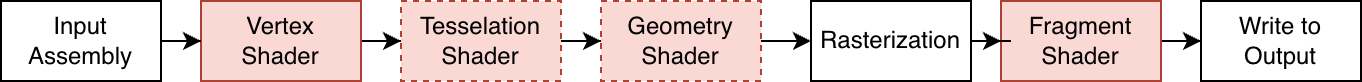
\includegraphics[scale=0.25,keepaspectratio]{RasterizationPipeline.drawio.png}

\caption{The rasterization pipeline. Programmable stages are highlighted in red, with optional components outlined with dotted lines.\label{fig:rasterpipe}}  
\end{figure}

\label{sssec:rasterization}


\paragraph{Deferred Shading}

\subsubsection{The Raytracing Pipeline}

The raytracing pipeline, depicted in \autoref{fig:raytracepipe}, is a different pipeline that graphics programmers can opt to use that is optimized for raytracing workflows. Compared to the rasterization and compute pipelines, the raytracing pipeline allows the program to loop back and generate more shader invocations. Rays are generated by the Ray Generation Shader (RGS), which are then raycast into a hardware-accelerated bounding volume hierarchy (BVH) known as the acceleration structure, depicted in \autoref{fig:tlas}.

The primary advantage offered by the raytracing pipeline is the hardware acceleration of ray casts into the BVH, which was abused by Zhang et al. in their work on accelerating sparse matrix-matrix multiplications using the ray tracing pipeline \cite{zhangRTSpMSpMHarnessingRay2025}.

\begin{figure}
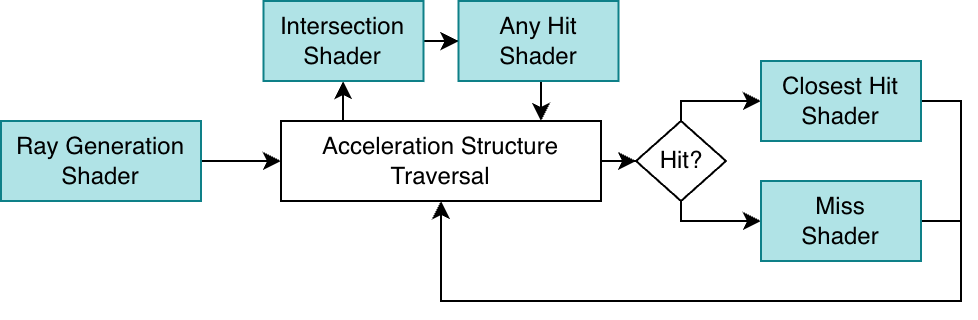
\includegraphics[scale=0.25,keepaspectratio]{RayTracingPipeline.drawio.png}
\caption{The ray tracing pipeline. Programmable stages are highlighted in green.\label{fig:raytracepipe}}  
\end{figure}
\begin{figure}
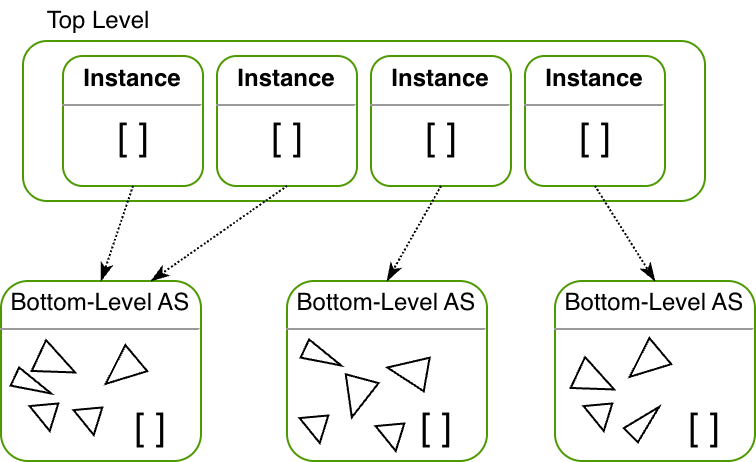
\includegraphics[scale=0.25,keepaspectratio]{AS.drawio.png}
\caption{The acceleration structure (AS) layout as described in Nvidia's DirectX 12 Raytracing tutorial\cite{DX12RaytracingTutorial}. The top-level acceleration structures (TLAS) instance the bottom-level acceleration structures (BLAS), not unlike how objects in a scene instance the same meshes. \label{fig:tlas}}  
\end{figure}

\subsection{Compilers in Computer Graphics}

Computer graphics as a field is huge, spanning different rendering techniques and the use of machine learning in various parts of the render pipeline. We will hence cover a small subset of it, relating to the use of compiler techniques in computer graphics.

\subsubsection{The Rendering Equation}
 
The rendering equation\cite{kajiyaRenderingEquation1986} refers to the equation used to compute the value of a point's irradiance, which we define in \autoref{eqn:rendering}. It computes the irradiance for a point by integrating over the hemisphere $\Omega$, taking in as input the normal at the point $\mathbf{n}$ and incoming and outgoing radiance $L_i$ and $L_o$ along the directions $\omega_i$ and $\omega_o$ respectively. $f$ most often appears as $f_r$, known as the bidirectional reflection function, which is the proportion of light reflectioned from $\omega_i$ to $\omega_o$.
\begin{align}
  \label{eqn:rendering}
  \int_\Omega L_i(\omega_i)f(\omega_i,\omega_o,\theta)\langle \mathbf{n}, \omega_i \rangle \mathsf{d} \omega_i
\end{align}

The integral over the hemisphere is what allows for computing global illumination in a realistic manner. By nature of being an integral over a 2D manifold, it is also computationally intensive, yet must be performed for every fragment in the render target to achieve realistic lighting. In real-time workflows, this is approximated by using radiance probes to cache global illumination, or by using the raytracing pipeline.

\subsubsection{Domain Specific Languages (DSLs) for Computer Graphics}
A number of DSLs have been devised for computer graphics. Many if not all of these DSLs target raytracing workloads, with very few options for a DSL targeting real-time rendering.

\subsubsection{Inverse Rendering}

Inverse rendering derives geometry and materials from one or more final images of a target scene. This is achieved through machine learning; specifically, the approach of \emph{differentiable rendering} uses automatic differentiation of the shaders to produce geometry and textures that would produce the same target images. State of the art in the field includes Mitsuba (and its underlying IR, DR.JIT\cite{jakobDRJITJustintimeCompiler2022}), which is able to automatically differentiate the whole pipeline and train for both geometry and render simultaneously, and SlangD\cite{bangaruSLANGDFastModular2023}, which performs automatic differentiation at the per-shader level which improves performance but forces geometry and render to be trained for separately. We include this as an interesting exploration of compiler techniques in computer graphics, and an avenue for potential research in the future.

\section{Progress Report}

\section{Thesis Proposal}

The programmable deliverable of this thesis is to develop an MLIR dialect for dispatching work to the GPU. The research value of such a project is not immediately apparent, however, it does lay the groundwork and an overarching research theme for research ideas exploring cross-pipeline optimizations. In the short term, the concrete paper ideas are:
\begin{itemize}
  \item Compiling to Accelerate Block-Sparse Linear Algebra with Raytracing Hardware
  \item Rasterization Pipeline Optimizations as Program Rewrites
\end{itemize}

\subsection{Compiling to Accelerate Block-Sparse Linear Algebra with Raytracing Hardware}

Target Venue: ASPLOS 

The general idea of tackling linear algebra as a geometry problem is not a particularly novel innovation. Why, even dense GEMM is often modelled as a polyhedral program. Therefore, the idea of modelling sparse-sparse matrix multiplication as a geometric problem should not come as a surprise either. By converting the elements of sparse matrices into triangles and utilizing the ray tracing pipeline's acceleration structure, Zhang et al.~\cite{zhangRTSpMSpMHarnessingRay2025} manage to harness the ray tracing hardware to optimize the sparse linear algebra problem, achieving a 1.85x speedup over cuSPARSE.

We observe that Zhang's approach uses OptiX, Nvidia's SDK for ray tracing, and posit that their approach can still be further refined by treating the lowering of the sparse computation to the raytracing pipeline as a compiler optimization. We will attempt to use compiler techniques to not only simplify the writing of the dispatch for the frontend programmer, but also enable well-known optimizations such as block-sparse formats. The block semantics available to block-sparse matrices more easily permit tensor core acceleration, and as geometric primitives with larger volume, should be more efficiently handled by the bounding volume acceleration structures. This approach is clearly cross-pipeline, utilizing both the compute and raytracing pipelines to optimize a linear algebra problem, and is simple to implement and explore with existing tools, allowing us to dedicate engineering effort to building a well-rounded GPU dispatch framework.

\subsection{Rasterization Pipeline Optimizations as Program Rewrites}

Target Venue: SIGGRAPH / SIGGRAPH ASIA

The rasterization pipeline is a well-understood programming model utilized by graphics engineers all across the video game industry. One of the most crucial optimizations one could perform to their graphics pipeline is to reduce the amount of overdraw in the scene, and a common way of doing this is with deferred shading. As stated in \autoref{sssec:rasterization}, deferred shading reduces overdraw by only performing the expensive lighting computations on fragments that are actually visible on the screen. While this reduces overdraw and usually results in a performance improvement, many intermediate textures (collectively known as the G-buffer or geometry buffer) must be materialized to cache the values for the lighting computation. This is both memory intensive and exhausts the limited texture units available in the hardware. To mitigate the latter, the classical approach is to pack the results into as few textures as possible, as each texture is able to store 4 separate values corresponding to the RGBA channels, and to utilize formats that reduce accuracy where it is not needed --- for instance, normals are typically stored in a 16 bit float format. A more effective approach to reducing memory overhead, and the one taken by most game engines, is to \emph{tile} the render parts, in a manner not unlike their compute counterparts.

We treat the tiling of the render pass as a program rewrite. Unlike linear algebra workloads, the iteration domain is not the only tiling target. The draw command's viewport and the frustum corresponding to the projection matrix must be tiled as well, respectively corresponding to pipeline and geometric semantics. By subdividing and rotating the frustum, however, the inter-tile depth buffer becomes incoherent, resulting in non-trivial adjustment for use in post-processing passes that rely on the depth buffer. One example of such a pass is depth-based edge detection. We will investigate the effects of tiling on the geometric semantics of the render pass, and attempt to resolve it with whole program optimization that is only possible with multi-level compilers. This will allow us to investigate the use of compiler rewrites as a means to optimize pipelines.

\subsection{Criteria for Success}

While adoption in the general community would be great, two years is hardly sufficient for a project to gain traction within the community. However, adoption by 

\section {Timeplan}
%% Bibliography
\bibliography{references}

\end{document}
